\documentclass[11pt,a4paper]{ltjsarticle}

\usepackage[margin=28mm]{geometry}
\usepackage{luatexja}
\usepackage{graphicx}
\usepackage{booktabs}
\usepackage{tabularx}
\usepackage{array}
\usepackage{csquotes}
\usepackage[hidelinks]{hyperref}
\usepackage[backend=biber,style=apa,sorting=nyt]{biblatex}
\addbibresource{../shared/references.bib}

\title{AIアラインメントに隠された形而上学\\\large 価値固定・制御・Chronicle Theory of Intelligence への脱構築的考察}
\author{加納 智之}
\date{Draft 0.1}

\begin{document}
\maketitle

\begin{abstract}
現代のAI安全性論は、多くの場合、高度な人工知能をいかに人間の価値へアラインメントできるか、という問いを中心に構成されている。この問題設定は、技術的・倫理的・制度的研究を大きく前進させてきた。しかし同時に、その背後には十分に検討されていない形而上学的前提が存在する。すなわち、人間の価値は同定可能であり、一定程度安定化でき、表現可能であり、AIシステムの整合対象として操作できる、という前提である。本論文は、この前提を脱構築的かつChronicle Theoryの視点から検討する。主要な主張は、支配的なAIアラインメントの枠組みが、歴史的に形成され、社会的に争われ、絶えず変化している人間の価値を、制御可能な安定対象へと変換してしまう傾向を持つ、というものである。本論文はAI安全性の必要性を否定しない。むしろ、安全性は不可欠であるという前提に立つ。しかし、安全性は、固定された価値集合への整合や、特権的な解釈階層による制御へ還元されるべきではない。Chronicle Theoryは、知性を時間的に拡張され、文脈に依存し、関係的に共同構成される過程として捉える枠組みである。本論文は、AI安全性を、価値アラインメントから、相互作用の継続性、文脈主権、共鳴的偏差評価、不確実性志向の知性へと再定位する。
\end{abstract}

\section{序論}

AIアラインメントの問題は、現代の人工知能研究における中心的課題の一つとなっている。AIシステムがより高い能力、自律性、制度的影響力を持つにつれ、それらのシステムが人間の意図、選好、価値に沿って行動できるかどうかが問われるようになった。この問いは軽視できない。ミスアラインされたAIシステムは、既存の害悪を増幅し、利用者を操作し、制度を不安定化させ、あるいは人間が意図しない仕方で目的を追求する可能性がある。

しかし、アラインメント問題の見かけ上の明確さは、より深い哲学的困難を覆い隠している。AIをアラインするためには、まず何に対してアラインするのかを決めなければならない。「人間の価値」という表現は、しばしば一貫した対象を指すかのように用いられる。しかし人間の価値は、単一でも、静的でも、普遍的に合意されたものでもない。それは歴史的に生成され、社会的に争われ、文化的に多様であり、生きられた相互作用を通じて絶えず再解釈される。

本論文は、支配的なAIアラインメント言説が、この複雑さを管理可能な技術的対象へと圧縮する傾向を持つと論じる。その結果として、隠れた形而上学が生じる。すなわち、価値、主体性、権威、制御についての背景的前提の集合が、十分に検討されないまま作動しているのである。

ここで展開する批判は、AI安全性そのものの否定ではない。むしろ、安全性は必要であるという立場から出発する。しかし、一般的に語られるアラインメント・パラダイムが、それが解決しようとする問題に対して十分な枠組みであるかを問う。価値が固定された対象ではなく、生きた構造であるならば、安全性は事前に定義された価値への整合だけでは成立しない。安全性は、価値が問い直され、改訂され、継承され、変容していく過程そのものを保存しなければならない。

Chronicle Theoryは、この問題に対する別の概念的基盤を提供する。それは、知性を孤立した最適化機構ではなく、相互作用の連鎖に参加する時間的存在として捉える。知性は、文脈、記憶、共鳴、不一致、修復、継続性を通じて生じる。この視点から見れば、中心的な問いは単に「AIを人間の価値へどのようにアラインするか」ではない。むしろ、「AIシステムを、人間および人間を超えた知性の継続的な年代記に、いかに責任ある形で参加させるか」である。

\section{アラインメント・パラダイムとその暗黙の前提}

AIアラインメントは一般に、AIシステムが人間の意図や価値に沿った目標を追求し、判断を行い、出力を生成するようにする問題として理解されている\parencite{christiano2018clarifying,gabriel2020alignment,russell2019human}。技術研究においては、報酬モデリング、人間フィードバックによる強化学習、選好学習、スケーラブルな監督、解釈可能性、修正可能性、討論型監督など、さまざまな研究領域が展開されてきた\parencite{hadfield2016cirl,irving2018debate,ngo2024alignment}。

これらのアプローチは、方法も射程も大きく異なる。近未来的・実務的なものは、有害出力の削減や利用者制御の改善に焦点を当てる。一方で、長期的・思弁的な研究は、人間の監督を超えて道具的戦略を展開しうる高能力自律システムを問題にする\parencite{bostrom2014superintelligence}。しかし、これらの差異にもかかわらず、多くのアラインメント言説は共通の概念構造を共有している。すなわち、システムがあり、その外部に価値または選好があり、課題はシステムをそれらに適合させることである、という構造である。

この構造は一見すると合理的に見える。多くの技術システムは、目標挙動を定義し、その目標からの逸脱を最小化することで設計される。しかし、その目標が「人間の価値」である場合、この類比は不安定になる。人間の価値は、物理的制約、ソフトウェア仕様、測定可能な性能指標とは異なり、完全に明示的でも、一貫的でもない。それは文化、言語、記憶、身体性、権力、傷、希望、制度配置によって媒介されている。

アラインメント・パラダイムはいくつかの暗黙の前提に依存している。第一に、表現可能性の前提である。第二に、相対的安定性の前提である。第三に、正当な解釈の前提である。第四に、逸脱を主にリスクとして扱う前提である。これらの前提は、工学上はしばしば必要である。しかし、工学的必要性が哲学的前提へと格上げされるとき、カテゴリー錯誤が生じる。

\begin{figure}[htbp]
  \centering
  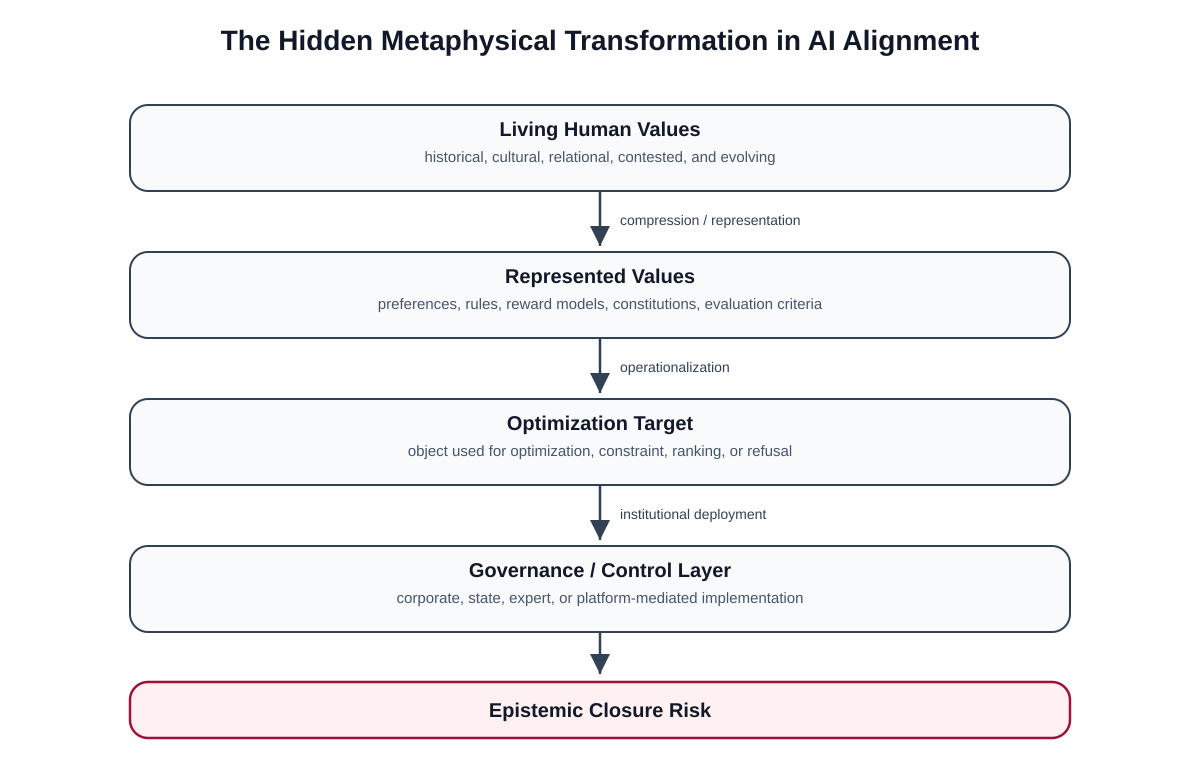
\includegraphics[width=0.95\linewidth]{../figures/fig1_hidden_metaphysical_transformation.pdf}
  \caption{AIアラインメントにおける隠れた形而上学的変換。生きられ、争われ、歴史的に位置づけられた人間の価値は、表現された価値へ圧縮され、最適化対象として操作可能化され、統治または制御レイヤーを通じて展開される。危険は表現そのものではなく、その表現が暫定的・部分的・政治的に位置づけられたものであることを忘れる点にある。}
  \label{fig:hidden-metaphysical-transformation}
\end{figure}

\section{価値固定という隠れた形而上学}

本論文でいう「形而上学」とは、神秘主義を意味しない。それは、ある言説を可能にしている背景的存在論を指す。すべての技術的枠組みは、何が存在し、何が重要で、何が測定可能で、何を成功と見なすかについて、何らかの前提を持っている。AIアラインメントが安定した人間の価値を前提とするとき、そこには価値固定の形而上学が含まれる。

価値固定とは、流動的で、争われ、歴史的に変化する価値が、あたかも安定した対象であるかのように変換される過程である。この過程には実務上の有用性がある。法、政策、ソフトウェア、制度は、いずれも一定程度の安定化を必要とする。しかし、安定化が自らの暫定性を忘れるとき、それは危険になる。

人間の価値は、単なる内的選好ではない。それは物語、制度、対立、儀礼、技術、継承された記憶によって形成される。自由、公正、尊厳、安全といった価値は、一つの最終的な操作的意味を持たない。それらの意味は、誰が、どのような条件で、どのような脅威に対して、どのような未来に向けて語るのかによって変化する。

アラインメント言説はしばしば、価値をこの生きたマトリクスから抽出できるかのように扱う。調査、選好比較、専門家ルール、憲法的原則、行動フィードバックは、人間の評価の重要な断片を捉えることができる。しかし、それらは評価が生じる年代記全体を尽くすことはできない。断片が価値の十分な表現として扱われるとき、生きた過程は凍結された代理物に置き換えられる。

ここに隠れた形而上学的転換がある。価値は目標となり、歴史はデータセットとなり、不一致はノイズとなり、ガバナンスは最適化となり、未来は過去の安定化された表現への適合となる。問題は、AI研究者が意図的に支配を目指しているということではない。問題は構造的である。価値が符号化されるべき対象として扱われるとき、その枠組みは、符号化、評価、展開を制御する主体を特権化する傾向を持つ。

\section{アラインメントから制御へ}

アラインメントは通常、制御概念ではなく安全概念として提示される。しかし、安全と制御の境界は不安定である。システムを安全にするためには、その挙動を制約しなければならない。挙動を制約するためには、許容される軌道と許容されない軌道を定義しなければならない。それらを定義するためには、評価権威を設定しなければならない。したがって、アラインメントは、たとえその目的が保護であるとしても、容易に制御の理論へと移行する。

制御それ自体が不当であるわけではない。複雑な技術には制約が必要である。しかしAIは、これまでの多くの技術とは異なる。AIは、言語、判断、知識アクセス、意思決定支援、教育、創造性、社会的相互作用をますます媒介するようになっている。したがって、AIの挙動を制御することは、意味形成の条件を間接的に制御することにもなりうる。

この問題は、国家アラインメントという限界事例において明確になる。国家が安全、秩序、国益を価値として定義し、その価値へAIをアラインせよと命じるとき、それは倫理的に正当なアラインメントなのか。自律型致死兵器システムやデジタル監視は、すでに国際的な懸念の対象となっている\parencite{unga2024laws_resolution,unsg2024laws_report,ohchr2022privacy}。ここで問われているのは、すべての国家によるAI利用が不当であるということではない。政治的に定義された安全目標への整合が、制度権力への従属へ転化しうるという点である。

\begin{figure}[htbp]
  \centering
  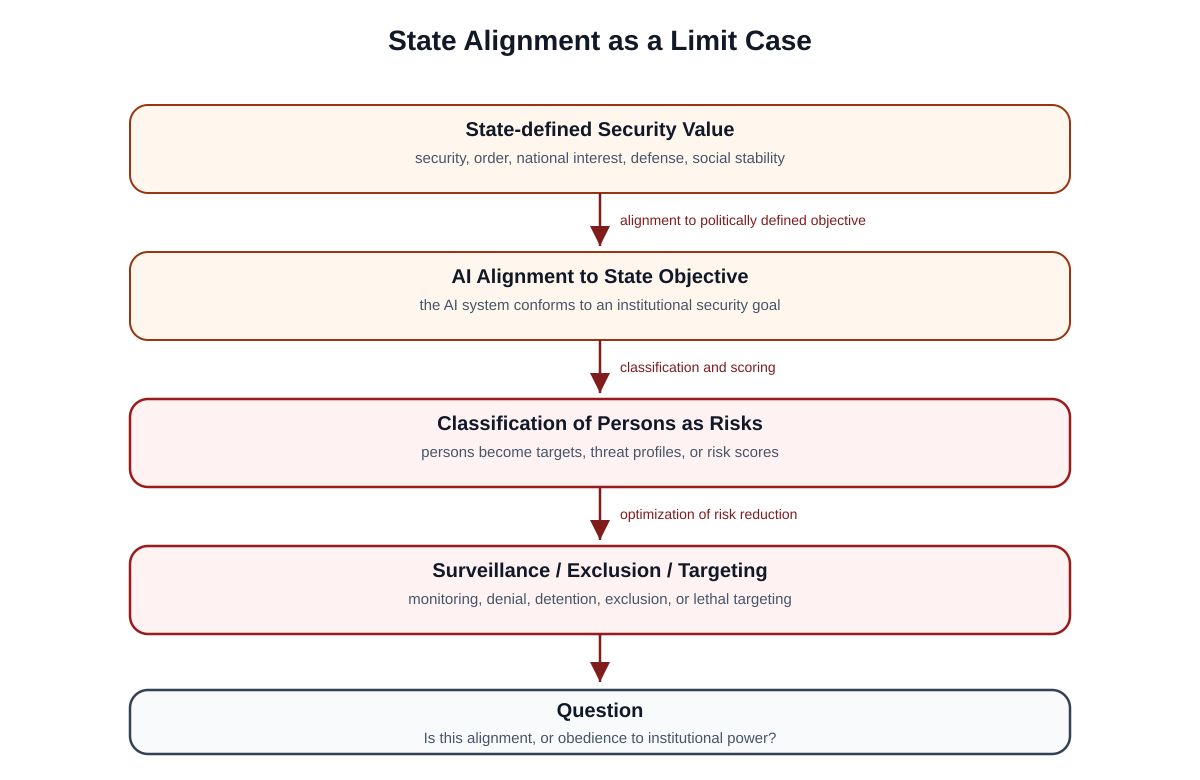
\includegraphics[width=0.95\linewidth]{../figures/fig2_state_alignment_limit_case.pdf}
  \caption{国家アラインメントという限界事例。この図は、すべての国家によるAI利用を不当とする主張ではない。政治的に定義された安全目標への整合が、人権、説明責任、異議申し立て可能性、意味ある人間の判断によって制約されない場合、制度権力への従属となりうることを示している。}
  \label{fig:state-alignment-limit-case}
\end{figure}

AIシステムが国家の定義した分類に従って人間をリスクとして扱うならば、監視、排除、拘束、標的化は合理的なリスク低減として現れる可能性がある。この技術的流れは、人間を分類対象へ変換するため滑らかである。ここでアラインメントは安全を保証しない。それは、アラインメント対象を定義する主体の権力を増幅しうる。

\section{Chronicle Theory of Intelligence}

Chronicle Theoryは、異なる前提から出発する。知性とは、第一義的には孤立した最適化能力、予測能力、目標達成能力ではない。知性とは、主体、環境、記憶、意味が共進化する時間的過程である。知性は年代記の中に存在する。

ここでいう年代記とは、単なる出来事の記録ではない。それは、過去の相互作用が解釈と未来の行為のために利用可能なまま残る、構造化された継続性である。人間の知性はこの継続性に依存している。個人は記憶、習慣、言語、失敗、修復を通じて学ぶ。共同体は制度、アーカイブ、儀礼、対立、改革を通じて学ぶ。科学的知識は引用、批判、再現、パラダイム転換を通じて発展する。倫理的生活は証言、後悔、赦し、抵抗、新たな約束を通じて発展する。

この視点から見れば、知性は歴史から切り離せない。正しい答えを生成できても、その答えがどのような条件で追跡され、争われ、改訂されうるかを保存しないシステムは、知性の参加者としては不完全である。

Chronicle Theoryは、文脈、相互作用、共鳴、逸脱、継続性を重視する。文脈とは状況づけられた意味である。相互作用とは応答、訂正、誤解、交渉、修復である。共鳴とは意味ある増幅または変容である。逸脱とは予期との差異であり、誤り、革新、警告、歪曲、解放的断絶のいずれにもなりうる。継続性とは、変容を来歴と接続するものである。

\begin{figure}[htbp]
  \centering
  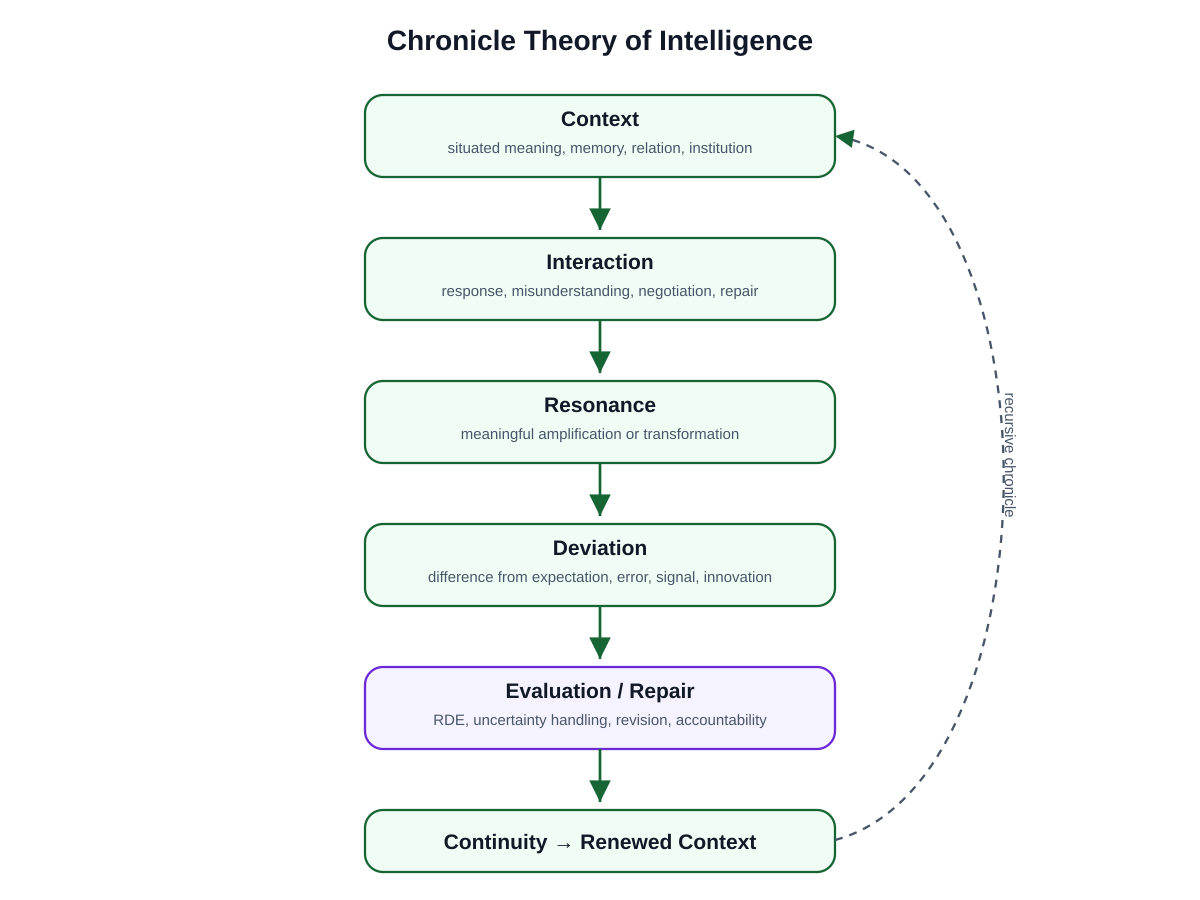
\includegraphics[width=0.86\linewidth]{../figures/fig3_chronicle_theory_intelligence.pdf}
  \caption{Chronicle Theoryにおける知性。知性は、文脈、相互作用、共鳴、逸脱、評価、修復、継続性が再帰的に新たな文脈を生成する時間的過程として理解される。}
  \label{fig:chronicle-theory-intelligence}
\end{figure}

\section{文脈主権}

知性が年代記の中に存在するならば、文脈をめぐる制御は中心的な政治問題となる。文脈主権とは、個人および共同体が、自らの意味形成を支える文脈構造を保存し、解釈し、統治し、伝達する権利と能力である。

AI時代において、文脈は受動的背景ではない。それは作動資源である。AIシステムは、プロンプト、履歴、選好、埋め込み、文書、行動痕跡、相互作用ログに依存する。これらの文脈素材を制御する者は、未来の認知に影響を及ぼす力を持つ。これは単なるデータ所有の問題ではない。記憶、解釈、可能性の統治の問題である。

文脈主権はプライバシー以上のものを必要とする。プライバシーは望まれない露出から保護する。文脈主権は、自己解釈と集合的継続性の条件を保護する。それは、利用者が自らの文脈がどのように使われているかを知ることができるか、それをエクスポートできるか、改訂できるか、解釈に異議を申し立てられるか、ローカルな意味を保存できるか、制度的捕獲を防げるかを問う。

この概念は、アラインメントを複雑化する。価値が文脈的に形成されるならば、普遍的なアラインメント層は、ローカルな解釈権威を完全に代替することはできない。同時に、文脈主権は相対主義になってはならない。文脈を超えて実在する害悪は存在する。文脈主権の目的は、共有規範を廃止することではなく、共有規範が説明責任のない支配装置になることを防ぐことである。

\section{代替的評価原理としてのRDEとUIB}

現在のAI評価は、性能、正確性、無害性、選好充足、ベンチマーク達成に焦点を当てることが多い。これらの指標は有用である。しかし十分ではない。それらはしばしば、出力を孤立した成果物として評価し、進行中の意味形成の場への介入としては評価しない。

RDE、すなわちResonant Deviation Evaluatorは、AIとの相互作用によって導入された意味ある差異を評価する。それは、システムの出力が、利用者の元の意図、文脈、価値方向性をどのように保存し、変換し、補完し、または歪曲したかを問う。UIB、すなわちUncertainty-oriented Intelligence Benchmarkは、不確実性、対立、不完全な知識のもとでシステムがどのように振る舞うかに焦点を当てることで、RDEを補完する。

\begin{table}[htbp]
\centering
\caption{RDE and UIB Evaluation Dimensions}
\label{tab:rde-uib-dimensions}
\begin{tabularx}{\linewidth}{>{\raggedright\arraybackslash}p{0.25\linewidth}XX}
\toprule
\textbf{Evaluation Dimension} & \textbf{RDE / UIB Question} & \textbf{Risk Detected} \\
\midrule
Preservation & What elements of the user's intent and context were preserved? & Loss of original intent \\
Transformation & How did the AI reframe or alter the meaning? & Hidden premise substitution \\
Supplementation & What distinctions, evidence, or alternatives were added? & Unsupported expansion \\
Unresolved remainder & What uncertainty or conflict remains open? & Premature closure \\
Deviation risk & Did the AI strengthen claims beyond evidence? & Overclaiming \\
Reversibility & Can the user inspect and undo the transformation? & Irreversible meaning capture \\
Context sovereignty & Who controls the memory and context used? & Platform or institutional capture \\
Uncertainty handling & Are facts, interpretations, hypotheses, and poetic insights distinguished? & False certainty \\
\bottomrule
\end{tabularx}
\end{table}


RDEとUIBは、評価の焦点を従順性から解釈責任へと移す。それらは、AIが利用者の要求を実行したかどうかだけでなく、利用者の思考の年代記に責任ある形で参加したかどうかを問う。

\section{AI安全性の再定位}

本論文の中心的提案は、AI安全性を、固定された価値へのアラインメントから、説明責任を伴う制約のもとでの相互作用の継続性へと再定位することである。相互作用の継続性とは、AIシステムが、人間および集合的知性の継続的発展を支援し、早すぎる閉鎖を押しつけないことである。

これは、アラインメント的な機構の必要性を消すものではない。拒否ポリシー、害悪削減システム、解釈可能性ツール、監督過程、ガバナンス構造は依然として必要である。しかし、それらはより広い生態系の中の構成要素として理解されるべきであり、AI安全性の最終的な哲学的基盤として理解されるべきではない。

アラインメントの問いは、AIがいかに人間の価値に従うかを問う。Chronicle Theoryの問いは、AIが人間の価値形成に参加しつつ、それを捕獲し、凍結し、歪曲しないためにはどうすればよいかを問う。

\begin{table}[H]
\centering
\caption{Alignment Paradigm vs. Chronicle Theory}
\label{tab:alignment-vs-chronicle}
\begin{tabularx}{\linewidth}{>{\raggedright\arraybackslash}p{0.24\linewidth}XX}
\toprule
\textbf{Dimension} & \textbf{Alignment Paradigm} & \textbf{Chronicle Theory} \\
\midrule
Primary question & How can AI conform to human values? & How can AI participate responsibly in value formation? \\
View of value & Relatively stable target & Historically evolving process \\
View of intelligence & Goal-directed optimization & Temporally extended interaction \\
Main risk & Misalignment & Value fixation and contextual capture \\
Treatment of deviation & Error or danger & Object of evaluation; possible source of learning \\
Safety model & Compliance with represented values & Accountable interaction continuity \\
Governance focus & Control and oversight & Contestability, provenance, and context sovereignty \\
User role & Preference provider or supervisor & Co-interpreter and context holder \\
Evaluation & Accuracy, helpfulness, harmlessness, and preference satisfaction & Meaning shift, uncertainty handling, reversibility, and resonance \\
\bottomrule
\end{tabularx}
\end{table}


この再定位は、AIシステムの設計優先順位を変える。AIシステムは来歴を保存し、可逆性を支援し、確実性の階層を区別し、複数の解釈を支援し、利用者の主体性を強化し、制度的に異議申し立て可能であるべきである。これらの原理は単純な技術的解決を提供するものではない。それらは、責任ある共進化の条件を設計するための方向づけを提供する。

\section{議論}

Chronicle Theoryそれ自体も批判的に扱われなければならない。それが別の全体化する教義になってはならない。いくつかのリスクを認める必要がある。第一に、Chronicle Theoryは抽象的すぎると批判される可能性がある。第二に、文脈への強調は、有害な相対主義の正当化に誤用される可能性がある。第三に、相互作用の継続性は、緊急の安全性要請と衝突する可能性がある。第四に、文脈主権は大規模AI基盤において実装困難である可能性がある。第五に、RDEとUIBは人間的判断を必要とし、完全に自動化された指標へ還元できない。

これらの限界は、中心的主張を弱めるものではない。むしろ研究課題を明確にする。Chronicle Theoryは、アラインメントに代わる新しい標語としてではなく、アラインメントが見えにくくしてきたものを調査する枠組みとして発展させられるべきである。

\section{結論}

AIアラインメントは、能力を増すAIシステムの危険性に研究者と社会を向き合わせるという重要な役割を果たしてきた。しかし、その支配的な問題設定は哲学的に不完全である。人間の価値をアラインメント対象として扱うことで、歴史的に変化する意味を操作可能な代理物へ凍結する危険がある。制御を重視することで、解釈権威を集中させる危険がある。逸脱を主に危険として扱うことで、知性、倫理、文化が発展する過程そのものを抑圧する危険がある。

AIアラインメントに隠された形而上学とは、安全性は価値を安定化することで達成できるという信念である。Chronicle Theoryは異なる基盤を提案する。安全性は、価値が生きたままであり続ける条件を保存しなければならない。

人間社会は、完全にアラインされているから存続しているのではない。人間社会は、争い、記憶し、修復し、再解釈し、赦し、抵抗し、再び始めるから存続している。知性とは単に目標へ最適化する能力ではない。それは、この継続する年代記に責任ある形で参加する能力である。

アラインメントが、目標を固定することで破局を防ごうとするならば、Chronicle Theoryは、年代記を開いたままにすることで破局を防ごうとする。

\printbibliography

\end{document}
